\documentclass[10pt]{report}
\usepackage{/Users/bradenhoagland/latex/math}

\lhead{Braden Hoagland}
\chead{Differential Geometry}
\rhead{}

\begin{document}
\tableofcontents

%+-------------------+
%| +---------------+ |
%| |    Chapter    | |
%| +---------------+ |
%+-------------------+
% Calculus on Euclidean Space

\chapter{Calculus on Euclidean Space}

%%%%%%%%%%%%%%%%%%%%
% Differentiable Functions
%%%%%%%%%%%%%%%%%%%%

\section{Differentiable Functions}

The \textbf{coordinate functions} are maps from $\mathbb{R}^n$ to $\mathbb{R}$, essentially picking out a single coordinate. They are given by
\begin{align*}
	x_i : \mathbb{R}^n &\to \mathbb{R} \\
	\mathbf{p}&\mapsto \mathbf{p}_i.
\end{align*}
If I'm working in $\mathbb{R}^3$, I'll probably use $x,y,$ and $z$ instead of $x_1, x_2,$ and $x_3$.

We say that a function $f:\mathbb{R}^n \to \mathbb{R}$ is \textbf{differentiable} if $f$ can be written as $f(x_1, x_2, \dots, x_n)$ and all partial derivatives of all orders exist and are continuous. A differentiable function is also called a \textbf{scalar field}.

The set of all differentiable functions/scalar fields forms a ring, so we can perform basic arithmetic with them.


%%%%%%%%%%%%%%%%%%%%
% Tangent Vectors and Vector Fields
%%%%%%%%%%%%%%%%%%%%

\section{Tangent Vectors and Vector Fields}

\begin{defn}
	Let $\mathbf{p} \in \mathbb{R}^n$. Then the \textbf{tangent space} $T_\mathbf{p}(\mathbb{R}^n)$ of $\mathbb{R}^n$ at $\mathbf{p}$ is the set of all tangent vectors in $\mathbb{R}^n$ originating at $\mathbf{p}$. The collection of all tangent spaces of $\mathbb{R}^n$ is the \textbf{tangent bundle} $T(\mathbb{R}^n)$ of $\mathbb{R}^n$.
\end{defn}

\begin{figure}[H]
	\centering
	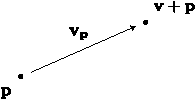
\includegraphics[scale=1]{fig/tan-vec.pdf}
	\caption{A tangent vector $\mathbf{v}_{\mathbf{p}}$ of $\mathbf{p}$ is an element of $T_{\mathbf{p}}(\mathbb{R}^n)$, and it's just the arrow from $\mathbf{p}$ to $\mathbf{p}+\mathbf{v}$.}
\end{figure}

If we define addition by $\mathbf{v}_{\mathbf{p}}+\mathbf{w}_{\mathbf{p}} \doteq (\mathbf{v}+\mathbf{w})_\mathbf{p}$ and scalar multiplication by $\lambda \mathbf{w}_\mathbf{p} \doteq (\lambda \mathbf{w})_\mathbf{p}$, then $T_\mathbf{p}(\mathbb{R}^n)$ becomes a vector space.

We say two tangent vectors $\mathbf{v}_\mathbf{p}$ and $\mathbf{w}_{\mathbf{q}}$ are equal if $\mathbf{v}=\mathbf{w}$ and $\mathbf{p}=\mathbf{q}$. We say they are parallel if $\mathbf{v}=\mathbf{w}$.

\begin{prop}
	$T_\mathbf{p}(\mathbb{R}^n)$ is isomorphic to $\mathbb{R}^n$.
\end{prop}
\begin{proof}
	Consider the function $\mathbf{v} \mapsto \mathbf{v}_\mathbf{p}$. This is clearly a one-to-one function from $\mathbb{R}^n$ onto $T_\mathbf{p}(\mathbb{R}^n)$. Additionally, it is clearly a homomorphism from the way we defined addition and scalar multiplication.
\end{proof}

\begin{defn}
	A \textbf{vector field} $V$ on $\mathbb{R}^n$ is a function
	\[
		V:\mathbb{R}^n \to T_{\mathbf{p}}(\mathbb{R}^n).
	\] 
\end{defn}

\begin{figure}[H]
	\centering
	\includegraphics[scale=0.3]{fig/vec-field.pdf}
	\caption{A vector field on $\mathbb{R}^2$ given by $\mathbf{p}\mapsto \mathbf{p}_{\mathbf{p}}.$}
\end{figure}

Vector fields can be added and scalar multiplied in the usual way for functions.

Let $U_1, \dots, U_n$ be vector fields on $\mathbb{R}^n$ such that
\begin{align*}
	U_1(\mathbf{p}) &= (1, 0, 0 \dots)_\mathbf{p} \\
	U_2(\mathbf{p}) &= (0, 1, 0, \dots)_\mathbf{p},
\end{align*} etc. for all $\mathbf{p} \in \mathbb{R}^n$. Then $U_1, \dots, U_n$ collectively are called the \textbf{natural frame field} on $\mathbb{R}^n$. Note that $U_i$ is a unit vector field in the positive $x_i$ direction.

We can decompose a vector field, in a sense, into multiple scalar fields. The scalar fields act as coordinates for our vector field, and the basis is the natural frame field.

\begin{prop}
	Let $V$ be a vector field on $\mathbb{R}^n$, then there are unique real-valued functions $v_1, \dots, v_n$ on $\mathbb{R}^n$ such that
	\[
	V = \sum_{i=1}^{n} v_i U_i.
	\] 
\end{prop}
\begin{proof}
	Let $\mathbf{p} \in \mathbb{R}^n$ be arbitrary, then by definition, $V(\mathbf{p}) \in T_\mathbf{p}(\mathbb{R}^n)$, so for some scalar fields $v_1, \dots, v_n$, we have
	\begin{align*}
		V(\mathbf{p}) &= (v_1(\mathbf{p}), \dots, v_n(\mathbf{p})) \\
		     &= v_1(\mathbf{p})e_1 + \dots v_n(\mathbf{p})e_n \\
		     &= v_1(\mathbf{p}) U_1(\mathbf{p}) + \dots v_n(\mathbf{p}) U_n(\mathbf{p}).
	\end{align*}
	Since $\mathbf{p}$ was arbitrary, $V = \sum_{i=1}^{n} v_i U_i$. The uniqueness of the $v_i$ follows from the fact that we got them directly from the components of the map $V$.
\end{proof}

\begin{defn}
	The $v_i$ in the above proposition are the \textbf{Euclidean coordinate functions} of $V$.
\end{defn}

\begin{note}
	We say that a vector field is differentiable if its Euclidean coordinate functions are themselves differentiable. From now on, assume vector fields are differentiable.
\end{note}


%%%%%%%%%%%%%%%%%%%%
% Directional Derivatives
%%%%%%%%%%%%%%%%%%%%

\section{Directional Derivatives}

Vector fields can naturally be thought of as machines that transform scalar fields into scalar fields. Given some scalar field $f$ and a vector field $V$, the most obvious way to act on $f$ with $V$ would be to use the tangent vectors given by $V$ to calculate derivatives of $f$. This requires us to first define the derivative of a scalar field at a point $\mathbf{p}$ with respect to a tangent vector $\mathbf{v}_\mathbf{p}$.

\begin{defn}
	Let $f:\mathbb{R}^n \to \mathbb{R}$ be a scalar field, and let $\mathbf{v}_{\mathbf{p}} \in T_p(\mathbb{R}^n)$. Then
	\[
		\mathbf{v}_{\mathbf{p}}[f] \doteq \frac{d }{d t} f(\mathbf{p}+t\mathbf{v}) \Big|_{t=0}
\] is the \textbf{directional derivative} of $f$ at $\mathbf{p}$ in the direction of $\mathbf{v}$. Note that it is a real number.
\end{defn}

\begin{prop}
	\label{prop:dir-der}
	Let $\mathbf{v}_\mathbf{p} \in T_\mathbf{p}(\mathbb{R}^n)$, then
	\[
		\mathbf{v}_{\mathbf{p}}[f] = \sum_i v_i \frac{\partial f}{\partial x_i} (\mathbf{p}).
	\] 
\end{prop}
\begin{proof}
	Since $\frac{d }{d t} (p_i + tv_i) = v_i$, we can use the chain rule to get
	\begin{align*}
		\frac{d }{d t} f(\mathbf{p}+t\mathbf{v}) \Big|_{t=0} &= \sum_{i} v_i \frac{\partial f}{\partial x_i} (\mathbf{p}+t\mathbf{v}) \Big|_{t=0} \\
						   &= \sum_i v_i \frac{\partial f}{\partial x_i} (\mathbf{p}).
	\end{align*}
\end{proof}

\begin{thrm}
	\label{thrm:props-of-dir-der}
	Let $f,g:\mathbb{R}^n \to \mathbb{R}$ be scalar functions, let $\mathbf{v},\mathbf{w} \in T_\mathbf{p}(\mathbb{R}^n)$, and let $\lambda,\eta\in\mathbb{R}$, then
	\begin{enumerate}
		\item $(\lambda \mathbf{v} + \eta \mathbf{w})[f] = \lambda \mathbf{v}[f] + \eta \mathbf{w}[f]$,
		\item $\mathbf{v}[\lambda f + \eta g] = \lambda \mathbf{v}[f] + \eta \mathbf{v}[g]$, and
		\item $\mathbf{v}[fg] = \mathbf{v}[f] g(\mathbf{p}) + f(\mathbf{p}) \mathbf{v}[g]$.
	\end{enumerate}
\end{thrm}
\begin{proof}
	It's straightforward to prove these by using Proposition \ref{prop:dir-der}.
\end{proof}

Parts (1) and (2) of this theorem say that $\mathbf{v}[f]$ is linear in both $\mathbf{v}$ and $f$. Part (3) is just the Leibniz rule.

It's easy to extend this idea to use a vector field instead of a fixed tangent vector. We simply use the vector field to map to a tangent vector, then use that to construct a directional derivative.

\begin{note}
In this sense, vector fields map scalar fields to scalar fields.
\end{note}

\begin{defn}
	The \textbf{operator} of a vector field $V$ on a scalar field $f$ is itself a scalar field
	\begin{align*}
		V[f]: \mathbb{R}^n &\to \mathbb{R} \\
		\mathbf{p} &\mapsto V(\mathbf{p})[f].
	\end{align*}
	This is the derivative of $f$ at the point $\mathbf{p}$ in the direction of $V(\mathbf{p})$.
\end{defn}

\begin{ex}
If $\left\{ U_i \right\}_{i=1}^n$ is the natural frame field on $V$, then $U_i[f] = \frac{\partial f}{\partial x_i} .$
\end{ex}

\begin{cor}
	Let $V,W$ be vector fields on $\mathbb{R}^n$, let $f,g,h:\mathbb{R}^n \to \mathbb{R}$ be scalar fields, and let $\lambda,\eta \in \mathbb{R}$, then
	\begin{enumerate}
		\item $(fV+gW)[h] = fV[h] + gW[h]$,
		\item $V[\lambda f+\eta g] = \lambda V[f] + \eta V[g]$, and
		\item $V[fg] = V[f] g + f V[g]$.
	\end{enumerate}
\end{cor}
\begin{proof}
	It's straightforward to prove these by using the corresponding part of Theorem \ref{thrm:props-of-dir-der}.
\end{proof}

Note that a ``scalar" in part (1) of this corollary can be a function, but the scalars must be actual numbers in part (2). That's because in part (1), the functions $f$ and $g$ get evaluated at some point $\mathbf{p}$, which yields a real number. In part (2), the only thing that gets evaluated at $\mathbf{p}$ is $V$, not anything in brackets.

%%%%%%%%%%%%%%%%%%%%
% Parameterized Curves
%%%%%%%%%%%%%%%%%%%%

\section{Parameterized Curves}

\begin{defn}
A \textbf{curve} in $\mathbb{R}^n$ is a differentiable function $\alpha:I\to \mathbb{R}^n$, where $I$ is an open interval in $\mathbb{R}$.
\end{defn}

Although curves could be defined without the condition that $I$ is open, it makes defining derivatives (which we'll do soon) easier. Without open intervals, we'd have edge cases where some derivatives need to be defined with one-sided limits, and we'd rather just avoid that altogether.

\begin{ex}{}{}
If $\alpha_i = p_i + t q_i$ for some points $\mathbf{p}$ and $\mathbf{q}$, then $\alpha$ is a line.
\end{ex}

\pagebreak

\begin{ex}
	To draw a helix, we can parameterize a curve $\alpha:\mathbb{R}\to \mathbb{R}^3$ by 
	\[
		\alpha(t)=(a \cos t, a \sin t, bt),
	\] where $a, b\neq 0$.
\end{ex}

\begin{defn}
Let $\alpha:I\to \mathbb{R}^n$ be a curve. Then for every $t \in I$, the \textbf{velocity} of $\alpha$ at $t$ is the tangent vector
\[
	\alpha'(t) = \left( \frac{d \alpha_1}{d t} (t), \dots, \frac{d \alpha_n}{d t} (t) \right)_{\alpha(t)}
\] at the point $\alpha(t) \in \mathbb{R}^n$.
\end{defn}

We can write the velocity vector alternatively as $\alpha'(t) = \sum_i \frac{d \alpha_i}{d t} (t) U_i(\alpha(t))$.

\begin{figure}[H]
	\centering
	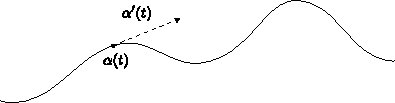
\includegraphics[scale=1]{fig/velocity.pdf}
	\caption{The velocity $\alpha'(t)$ is a vector tangent to $\alpha(t)$.}
\end{figure}


\begin{ex}
Using the parameterization of a helix from the previous example, its velocity vector is
\[
	\alpha'(t) = (-a \sin t, a \cos t, b)_{\alpha(t)}.
\]
\end{ex}

The velocity of a curve isn't determined by the shape of the curve, but rather by how quickly you travel the curve. To illuminate this, we consider reparameterizations of the same curve.

\begin{defn}
	Let $I$ and $J$ be open intervals, let $\alpha:I\to \mathbb{R}^n$ be a curve, and let $h:J\to I$ be differentiable. Then the curve $\beta:J\to \mathbb{R}^n$ given by the composition $\beta = \alpha \circ h$ is called a \textbf{reparameterization} of $\alpha$ by $h$.
\end{defn}

Let $\beta$ be a reparameterization of $\alpha$ by $h$. Then by the chain rule, its velocity vector is
\[
	\beta'(s) = h'(s) \alpha'(h(s)).
\] 
From this we see that unless $h$ has a constant derivative of 1, the velocities of $\alpha$ and $\beta$ will be different at the same point, even though they describe the same curve.

\begin{prop}
Let $\alpha$ be a curve in $\mathbb{R}^n$, and let $f:\mathbb{R}^n\to \mathbb{R}$ be differentiable. Then
\[
	a'(t)[f] = \frac{d (f(\alpha))}{d t} (t).
\] 
\end{prop}
\begin{proof}
	{\color{red}Go over notation of this with prof...}
	By definition,
	\[
		\alpha' = \left( \frac{d \alpha_1}{d t} , \dots, \frac{d \alpha_n}{d t}  \right)_{\alpha(t)},
	\] so by Proposition \ref{prop:dir-der},
	\[
		\alpha'(t)[f] = \sum_i \frac{d \alpha}{d t}  \frac{\partial f}{\partial x_i} (\alpha(t)).
	\] Noticing that the above expression is just an application of the chain rule, we can ``undo" the chain rule to get
	\[
		\alpha'(t)[f] = \frac{d (f(\alpha))}{d t} (t).
	\] 
\end{proof}

A curve $\alpha:\mathbb{R}\to \mathbb{R}^n$ is \textbf{periodic} if there is some $p>0$ such that $\alpha(t+p) = \alpha(t)$ for all $t$. The smallest such $p$ is then called the \textbf{period} of $\alpha$.

A curve whose velocity is nonzero at all points is called \textbf{regular}.


%%%%%%%%%%%%%%%%%%%%
% 1-Forms
%%%%%%%%%%%%%%%%%%%%

\section{1-Forms}

\begin{defn}
A \textbf{1-form} on $\mathbb{R}^n$ is a linear function
\[
	\phi:T(\mathbb{R}^n)\to \mathbb{R},
\] where $T(\mathbb{R}^n)$ is the tangent bundle of $\mathbb{R}^n$. For all $\mathbf{p}$, we can limit $\phi$ to
\[
	\phi_\mathbf{p}:T_{\mathbf{p}}(\mathbb{R}^n)\to \mathbb{R}.
\] 
\end{defn}

\begin{ex}
	The map $(v_1,v_2,v_3)_{\mathbf{p}}\mapsto v_1$ for all $\mathbf{p} \in \mathbb{R}^3$ is a 1-form.
\end{ex}

There's an equivalent way of formulating this that uses fancier vocab. If $\mathcal{V}$ is a vector space, then the set of all linear maps from $\mathcal{V}$ to $\mathbb{R}$ is itself a vector space. We call it the \textbf{dual space} of $\mathcal{V}$ and denote it by $\mathcal{V}^*$, and its elements are called \textbf{covectors}.

Thus a 1-form $\phi$ is an element of $T^*(\mathbb{R}^n)$. It can be limited to elements $\phi_\mathbf{p}$ of the \textbf{cotangent space} $T_{\mathbf{p}}^*(\mathbb{R}^n)$, in which cae we can also call $\phi_\mathbf{p}$ a \textbf{tangent covector}.

\begin{note}
Since vector fields produce tangent vectors and 1-forms map tangent vectors to real numbers, we can think of 1-forms as being dual to the notion of vector fields.
\end{note}

Addition of 1-forms is defined pointwise. We can also define a sort of scalar multiplication with scalar fields. If $\phi$ is a 1-form and $f$ is a scalar field, define
\[
	(f\phi)(\mathbf{v}_{\mathbf{p}}) \doteq f(\mathbf{p}) \phi(\mathbf{v}_\mathbf{p})
\] for all $\mathbf{v}_{\mathbf{p}} \in T_\mathbf{p}(\mathbb{R}^n)$.

Given a vector field $V$, we can naturally act on it with a 1-form $\phi$ by
\begin{align*}
	\phi(V):\mathbb{R}^n&\to \mathbb{R} \\
	\mathbf{p}&\mapsto \phi(V(\mathbf{p})).
\end{align*}
Thus we can view 1-forms as operators that convert vector fields into scalar fields. Additionally, it is easy to show that 1-forms act linearly on vector fields.

If $\phi(V)$ is differentiable whenever $V$ is differentiable, then we say that $\phi$ itself is differentiable.

\begin{note}
From now on, assume any given 1-form is differentiable.
\end{note}

\begin{defn}
Let $f:\mathbb{R}^n\to \mathbb{R}$ be differentiable. Then the \textbf{differential} $df$ of $f$ is the 1-form such that
\[
	df(v) = \mathbf{v}_{\mathbf{p}}[f]
\] for all tangent vectors $\mathbf{v}_{\mathbf{p}}$ of some point $\mathbf{p} \in \mathbb{R}^n$.
\end{defn}

Since $\mathbf{v}_{\mathbf{p}}[f]$ is a map from the tangent space to $\mathbb{R}$, and since we proved earlier that it is linear for all $p$, $df$ is in fact a 1-form.

\begin{ex}
Consider the differentials $dx_1, \dots, dx_n$ of the natural coordinate functions on $\mathbb{R}^n$. For a tangent vector $\mathbf{v}_{\mathbf{p}}$ of a point $\mathbf{p}$, we have
\[
	dx_i(\mathbf{v}_{\mathbf{p}}) = \mathbf{v}_{\mathbf{p}}[x_i] = \sum_j v_j \frac{\partial x_i}{\partial x_j} (\mathbf{p}) = \sum_j v_j \delta_{ij} = v_i,
\] where $\delta_{ij}$ is the Kronecker delta. Thus $dx_i$ just extracts the $i$-th coordinate of a tangent vector, regardless of its point of application.
\end{ex}

We can now go about classifying all possible 1-forms. Since every $dx_i$ is a one-form, any function of the form
\[
\sum_i f_i \;dx_i
\] is also a 1-form. As it turns out, this describes every possible 1-form. The $f_i$ for a particular 1-form are determined by where that form sends the natural frame field, similar to how linear functions are determined by where they send basis elements.

\begin{prop}
Let $\phi$ be a 1-form, then
\[
	\phi = \sum_i f_i \;dx_i,
\] where $f_i = \phi(U_i)$.
\end{prop}
\begin{proof}
	Since $\mathbf{v}_{\mathbf{p}} = \sum_i v_i U_i(\mathbf{p})$ and since $\phi$ is linear, we have
	\begin{align*}
		\phi(\mathbf{v}_{\mathbf{p}}) &= \phi\left( \sum v_i U_i(\mathbf{p}) \right) \\
					      &= \sum \phi(U_i(\mathbf{p}))v_i \\
					      &= \sum f_i(\mathbf{p}) v_i \\
					      &= \left( \sum f_i \;dx_i \right)(\mathbf{v}_{\mathbf{p}}).
	\end{align*}
\end{proof}

\begin{defn}
The $f_i$ above are called the \textbf{Euclidean coordinate functions} of $\phi$.
\end{defn}

\begin{cor}
	\[ df = \sum_i \frac{\partial f}{\partial x_i} dx_i.\]
\end{cor}
\begin{proof}
	$df(U_i) = U_i[f] = \frac{\partial f}{\partial x_i} .$
\end{proof}

{\color{red}Bottom of pg 25 to top of pg 27.}

%%%%%%%%%%%%%%%%%%%%
% Differential Forms
%%%%%%%%%%%%%%%%%%%%

\section{Differential Forms}

1-forms are part of a larger family of differential forms. 0-forms are just scalar fields, 1-forms are of the form $\sum f_i \;dx_i$, and we can get all other $n$-forms through multiplication of other forms.

Define the wedge product ... {\color{red}(do this.)} The only unusual rule that the wedge product must follow is anti-commutativity:
\[
\phi \wedge \psi = - \psi \wedge \phi.
\] 

\begin{ex}
A direct consequence of anti-commutativity is that two 1-forms wedged together is the zero map:
\[
\phi\wedge\phi = 0.
\] 
\end{ex}

\begin{note}
I might write $dx_i \wedge dx_j$ as $dx_i\;dx_j$ for simplicity.
\end{note}

We can generalize the differential to apply to more than just scalar fields (0-forms). Given any form
\[
\varphi = \sum_{I} f_I \;dx_I,
\] we define $d\varphi)$ by
\[
	d\varphi \doteq \sum_{I} d(f_I)\wedge \;dx_I.
\] 
Thus we can view the $d$ operator as converting an $n$-form to an $(n+1)$-form, and we call it the \textbf{exterior derivative}.

{\color{red}Stuff about how this generalizes div, grad, and curl...}

%%%%%%%%%%%%%%%%%%%%
% Mappings
%%%%%%%%%%%%%%%%%%%%

\section{Mappings}

In general, we can have functions $F:\mathbb{R}^n\to \mathbb{R}^m$, which are given by $m$ real-valued functions of $n$ variables each. We call differentiable such functions \textbf{mappings}.

\begin{defn}
The \textbf{tangent map} $F_*$ of a mapping $F:\mathbb{R}^n\to \mathbb{R}^m$ is a map
\[
	F_* : T(\mathbb{R}^n) \to T(\mathbb{R}^m)
\] between the tangent bundles of $\mathbb{R}^n$ and $\mathbb{R}^m$. In particular, at any point $\mathbf{p}$, the tangent map can be limited to the function
\[
	F_{*\mathbf{p}}:T_{\mathbf{p}}(\mathbb{R}^n)\to T_{F(\mathbf{p})}(\mathbb{R}^m)
\]
given by mapping $\mathbf{v}_{\mathbf{p}}$ to the initial velocity of the curve $t\mapsto F(\mathbf{p}+t\mathbf{v})$.
\end{defn}

\begin{figure}[H]
	\centering
	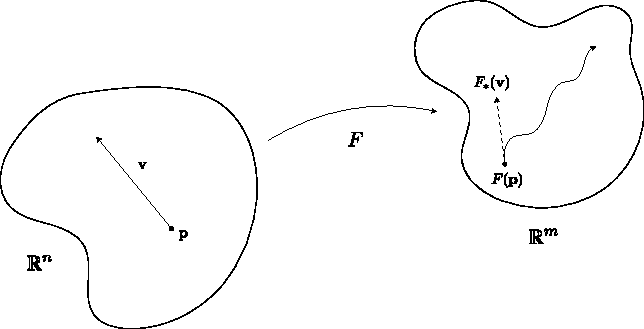
\includegraphics[scale=1]{fig/tan-map.pdf}
	\caption{The tangent map $F_*$ maps tangent spaces to tangent spaces by using the velocity of a curve.}
\end{figure}

The defintion requires us to use the \textit{initial} velocity because even though we're starting with a line in $\mathbb{R}^n$, its image under $F$ might be all curvy.

\begin{prop}
	Let $F=(f_1, \dots, f_m)$. If $\mathbf{v} \in T_{\mathbf{p}}(\mathbb{R}^n)$, then
	\[
		F_{*}(\mathbf{v}) = (\mathbf{v}[f_1], \dots, \mathbf{v}[f_m])_{F(\mathbf{p})}.
	\] 
\end{prop}
\begin{proof}
	Consider the curve $\beta$ traced out by $F(\mathbf{p}+t\mathbf{v})$, then
	\[
		\beta(t) = (\dots, f_i(\mathbf{p}+t\mathbf{v}), \dots).
	\] $F_{*}(\mathbf{v})$ is just $\beta'(0)$, so we calculate it as
	\[
		\beta'(0) = \left( \dots, \frac{d }{d t} f_i(\mathbf{p}+t\mathbf{v}) \Big|_{t=0}, \dots \right)_{\beta(0)}.
	\] But each component is straight up the definition of the directional derivative, and $\beta(0) = F(\mathbf{p})$, so this becomes
	\[
		F_{*}(\mathbf{v}) = (\dots, \mathbf{v}[f_i], \dots)_{F(\mathbf{p})}.
	\] 
\end{proof}

This shows $F_*$ is linear, but it's more than just a linear map between tangent spaces. It's very deeply connected to the {\color{red}more subtle than this, I think...}Jacobian... in the sense that it actually is the Jacobian. The corollary below might look complicated, but all it's saying is that $F_*$ is the linear map given by the matrix $[\frac{\partial f_i}{\partial f_j} ]_{ij}.$

{\color{red}Actually calculate $F_{*\mathbf{p}}(\mathbf{v}_{\mathbf{p}})$. Does it involve multiplying a tangent vector by the Jacobian maybe?}

{\color{red}1-1 iff onto when linear transformation is between two vec spaces of same dim. Useful for showing when $F_{*\mathbf{p}}$ is an isomorphism.}

\begin{cor}
\[
	F_{*}(U_j(\mathbf{p})) = \sum_{j=1}^{m} \frac{\partial f_i}{\partial x_j} (\mathbf{p}) \overline{U}_{i}(F(\mathbf{p})),
\] where $\left\{ \overline{U}_i \right\}_{i=1}^m$ is the natural frame field on $\mathbb{R}^m$.
\end{cor}
\begin{proof}
	$U_j[f_i] = \frac{\partial f_i}{\partial x_j} .$
\end{proof}

\begin{note}
We can interpret $F_*$ at $\mathbf{p}$ as the best linear approximation to $F$ at $\mathbf{p}$.
\end{note}

\begin{defn}[]
A mapping $F$ is \textbf{regular} if $F_*$ is one-to-one at all $\mathbf{p}$.
\end{defn}

This isn't the only way to characterize a regular mapping. Since $F_*$ is linear, the following are equivalent:
\begin{enumerate}
	\item $F_*$ is everywhere one-to-one.
	\item $F_*(\mathbf{v}_{\mathbf{p}}) = 0$ implies $\mathbf{v}_{\mathbf{p}}=0.$ 
	\item The Jacobian of $F$ is full rank.
\end{enumerate}

\begin{defn}[]
	A \textbf{diffeomorphism} is a mapping that has a differentiable inverse.
\end{defn}

\begin{thrm}[Inverse Function Theorem]
Let $F:\mathbb{R}^n\to \mathbb{R}^n$ be a mapping between Euclidean spaces of the same dimension. If $F_*$ is one-to-one at $\mathbf{p}\in \mathbb{R}^n$, then there is an open neighborhood $U$ of $\mathbf{p}$ such that $F$ restricted to $U$ is a diffeomorphism onto some open set $V$.
\end{thrm}

This is saying that if we have a mapping from $\mathbb{R}^n$ to $\mathbb{R}^n$ that is one-to-one at a given point, then that mapping is locally invertible at that point.

%+-------------------+
%| +---------------+ |
%| |    Chapter    | |
%| +---------------+ |
%+-------------------+
% Frame Fields

\chapter{Frame Fields}

%%%%%%%%%%%%%%%%%%%%
% The Dot Product
%%%%%%%%%%%%%%%%%%%%

\section{The Dot Product}

Earlier we showed that $\mathbf{v}\mapsto \mathbf{v}_{\mathbf{p}} $ was an isomoprhism, so we can naturally extend the usual dot product to work in tangent spaces. Given $\mathbf{v}_{\mathbf{p}}, \mathbf{w}_{\mathbf{p}} \in T_{\mathbf{p}}(\mathbb{R}^n)$, we define their dot product to be
\[
\mathbf{v}_{\mathbf{p}}\cdot \mathbf{w}_{\mathbf{p}} = \mathbf{v} \cdot \mathbf{w}.
\] 

{\color{red}Get rid of use of $e_i$ earlier on?}


\end{document}
